\documentclass[tikz,border=8pt]{standalone}
\usepackage{amsmath,amssymb}
\usetikzlibrary{arrows.meta,positioning,calc}
\definecolor{TargetBlue}{HTML}{2364AA}
\definecolor{NuisanceOrange}{HTML}{E6862A}
\definecolor{EfficientGreen}{HTML}{278A64}
\definecolor{NeutralGray}{HTML}{68717C}
\tikzset{
  box/.style={draw=NeutralGray, very thick, rounded corners=2pt, fill=white,
    minimum height=9mm, inner xsep=7mm, align=center},
  implication/.style={-{Latex[length=3mm]}, very thick, TargetBlue},
  condition/.style={font=\small, fill=white, text=NeutralGray, inner sep=2pt}
}
\begin{document}
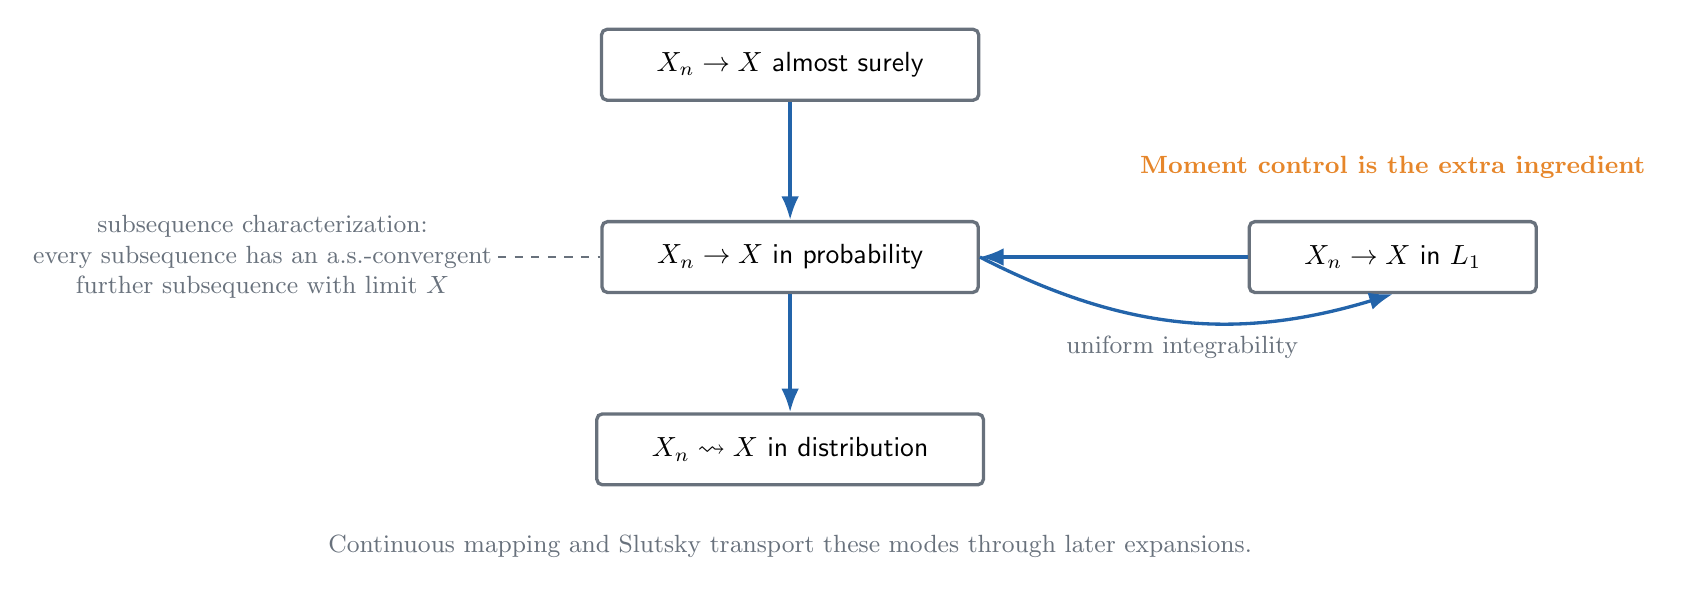
\begin{tikzpicture}[font=\sffamily, node distance=15mm and 24mm]
  \node[box] (as) {$X_n\to X$ almost surely};
  \node[box, below=of as] (prob) {$X_n\to X$ in probability};
  \node[box, below=of prob] (dist) {$X_n\rightsquigarrow X$ in distribution};
  \node[box, right=34mm of prob] (lone) {$X_n\to X$ in $L_1$};

  \draw[implication] (as) -- (prob);
  \draw[implication] (prob) -- (dist);
  \draw[implication] (lone) -- (prob);
  \node[condition, left=13mm of prob, align=center] (subseq)
    {subsequence characterization:\\every subsequence has an a.s.-convergent\\further subsequence with limit $X$};
  \draw[NeutralGray, dashed, thick] (subseq.east) -- (prob.west);
  \draw[implication, bend right=22] (prob.east) to node[condition, below=1mm]
    {uniform integrability} (lone.south);

  \node[above=4mm of lone, text=NuisanceOrange, align=center, font=\small\bfseries]
    {Moment control is the extra ingredient};
  \node[below=5mm of dist, text=NeutralGray, align=center, font=\small]
    {Continuous mapping and Slutsky transport these modes through later expansions.};
\end{tikzpicture}
\end{document}
